\section{Introduction}


% OC to ZSOC 등장까지
Object counting, which was initially studied for specific targets, e.g., crowds~\cite{h8}, cells~\cite{2018cell}, animals~\cite{2016animal}, and cars~\cite{2016cars}, has shown that the number of objects can be counted even within a dense image.
Furthermore, recent works have shown significant advances to infer the number of arbitrary objects with several human-annotated exemplar patches.
However, such a strong prerequisite that every cumbersome guidance must be equipped is undoubtedly the main challenge to overcome to grant applicability to object counting methods.
In this context, Zero-Shot Object Counting~(ZSOC) was proposed to mitigate the need for human labor.


\begin{figure}[t]
    \begin{center}
    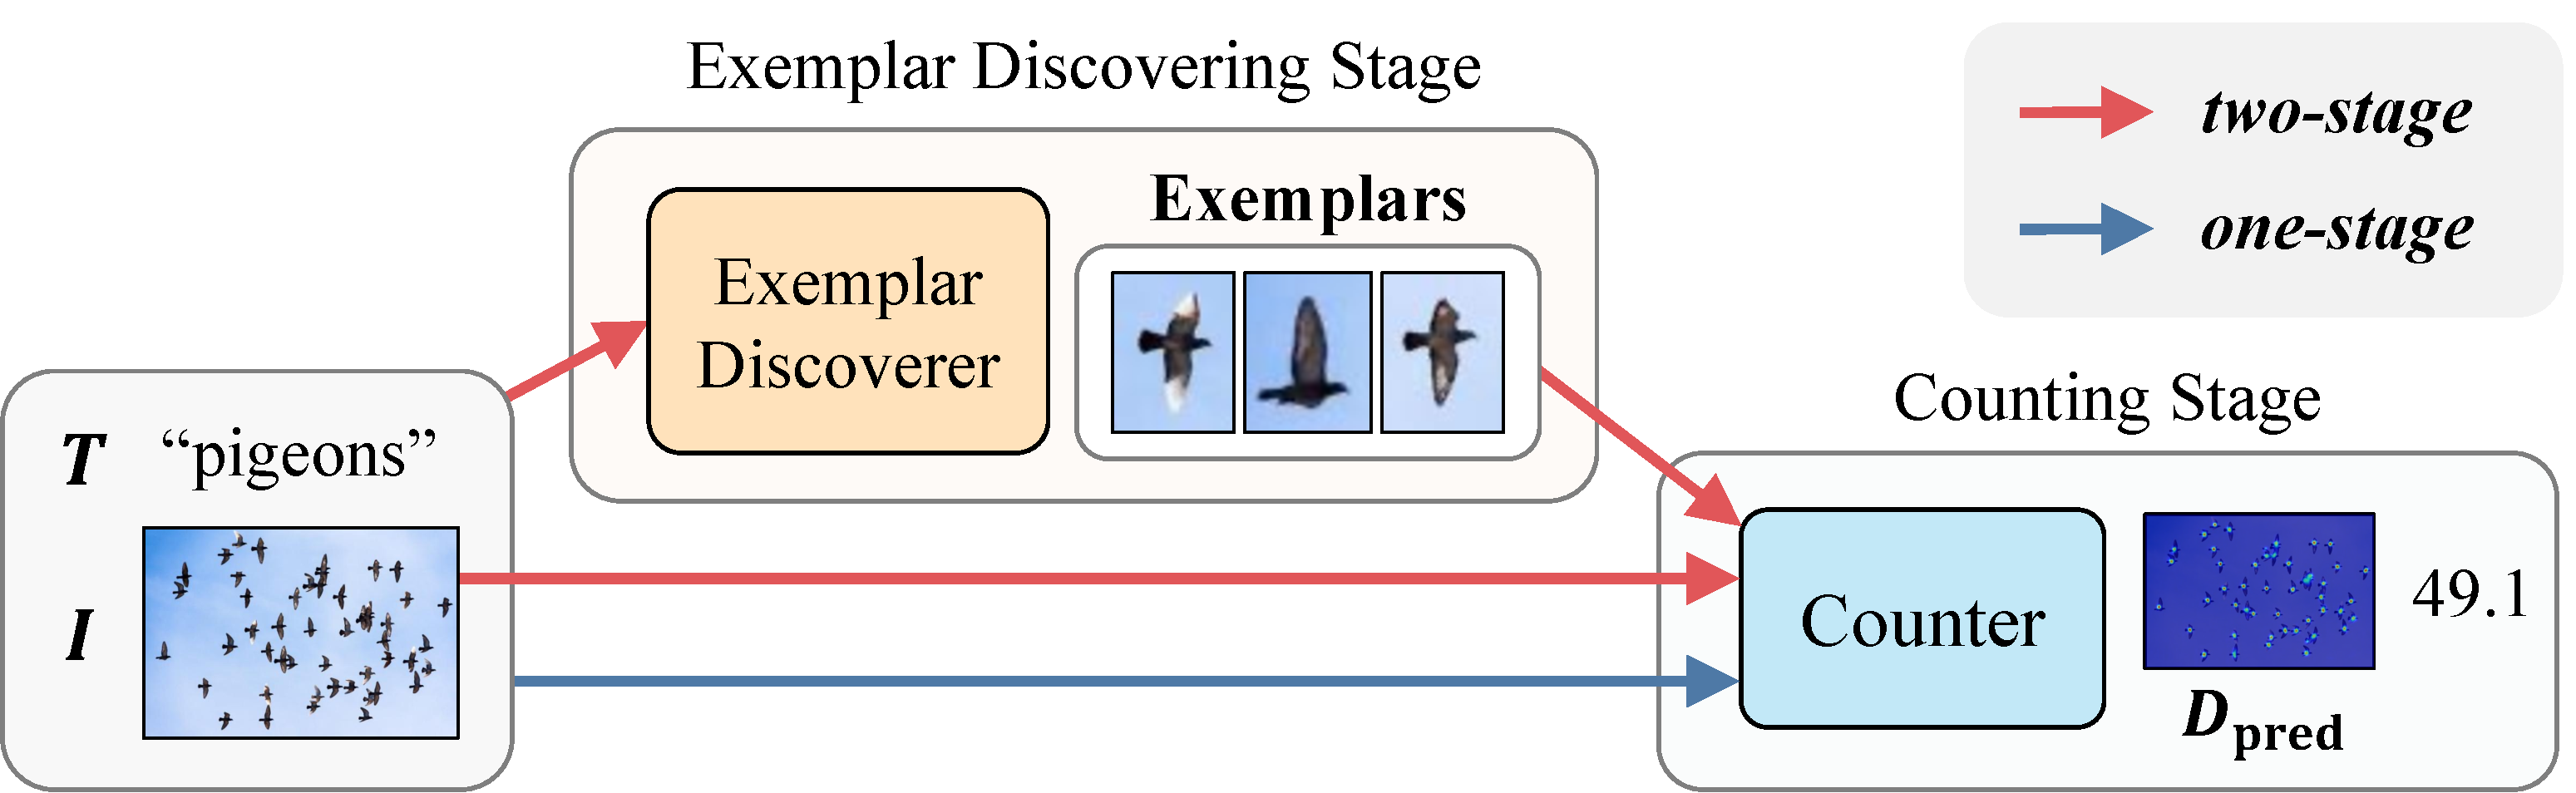
\includegraphics[width=\linewidth]{figs/intro_v3.pdf}
    \end{center}
    \caption{
        Comparison between two-stage pipeline and one-stage pipeline~(ours).
        The two-stage pipeline requires training the exemplar discoverer~(orange) before the counter~(blue), along with the need for an extra training dataset to optimize the discoverer.
        In contrast, our one-stage pipeline is designed to be simpler and does not necessitate any additional data or training stage. 
    }
    \label{fig:intro}
\end{figure}


% 기존 ZSOC는 2-stage라는 단점을 가짐
Current ZSOC approaches commonly adopt a two-stage pipeline as illustrated in Fig.~\ref{fig:intro}.
These works primarily focus on identifying exemplar patches within the image and subsequently adopt the counting framework from the literature of few-shot object counting~\cite{2022BMNet, 2021FAMNet}.
To identify the exemplar patches, RepRPN~\cite{2022RepRPN} considered the repetition score to detect object patches that frequently appear within the image.
Requirement for counting the desired classes over frequent ones, ZSC~\cite{2023zsc} utilized the class names to enable the class specification.
They localize exemplars by identifying the k-nearest neighbors of the class name embeddings among randomly cropped patches.
Despite their progress, the potential localization error propagation in the two-stage training pipeline~\cite{nag2022zero} is an untapped problem in ZSOC frameworks.
Indeed, they utilized additional datasets to train decent exemplar discovery networks.



% VLBase 설명
This paper pursues a simplified zero-shot object counting framework.
We instantiate an end-to-end ZSOC counter namely Visual-Language Baseline~(VLBase), which consists of a CLIP~\cite{2021clip} encoder and counting decoder.
By leveraging the embedding space of CLIP which enables the implicit association of the semantic and patch embeddings to localize the target object~\cite{2022maskclip, li2023clipsurgery}, VLBase eliminates the need for an exemplar discovery process.



% VLCounter 설명
Additionally, we introduce VLCounter which is built upon VLBase by incorporating three modules devised to tailor VLBase for object counting.
First, we propose Semantic-conditioned Prompt Tuning~(SPT) which extends the visual prompt tuning~(VPT) to efficiently finetune CLIP for the counting task.
Instead of utilizing na\"ive learnable prompts, SPT employs conditioning via semantic embedding to generate patch embeddings that emphasize the region of interest.
Subsequently, based on our observation that the similarity maps between patch embeddings obtained using SPT and semantic embeddings already provide a decent approximation of object locations, we employ simple Learnable Affine Transformation~(LAT) to adjust only the finer details.
Finally, to equip the decoder with the generalization capability and provide rich clues, we exploit intermediate features across different encoding layers of CLIP through Segment-aware Skip Connections~(SaSC).
With all components combined, our simple end-to-end one-stage framework records new state-of-the-art results on the FSC147~\cite{2021FAMNet} dataset validating its superiority over the previous ZSOC methods.
Moreover, we provide additional evidence of cross-dataset generalization by evaluating performance on the car counting dataset CARPK~\cite{2017drone}.

Our contributions are three-fold:
\begin{itemize}
    \item We instantiate an end-to-end baseline for ZSOC, VLBase, by exploiting the vision-language association capability of CLIP. 
    \item We propose a VLCounter consisting of SPT, LAT, and SaSC that allows the model to utilize the generalization capability of CLIP in a counting-specific manner.
    \item Our experiments on FSC147 and cross-dataset validation verify the effectiveness of VLCounter.
\end{itemize}